\chapter{Validierung}
\label{Validierung}

Ziel der Diplomarbeit ist die Entwicklung einer nutzerfreundliche Oberfläche zur Problemlösung in modularen Anlangen. Dieses Kapitel beantwortet, wie gut die Umsetzung geglückt ist. Dazu werden zunächst die Anforderungen an das Assistenzsystem ausgewertet. 

\section{Vergleich mit Anforderungen}
In Abschnitt \ref{3:Anforderungen} wurden Anforderungen an das Assistenzsystem gestellt. Die Erfüllung der Anforderungen wird im Folgenden diskutiert. Eine erste Einschätzung gibt jeweils eine Tabelle. Ein + bedeutet voll erfüllt, ein o bedeutet teilweise erfüllt und ein - bedeutet nicht erfüllt.

\subsection{Unterstützung der Problemidentifikation}
Der Nutzer soll bei der Problemidentifikation unterstützt werden. Tabelle \ref{tab:Anforderungen-Problemidentifikation} stellt dar, wie gut die einzelnen Anforderungen durch den Prototypen erfüllt sind.
\begin{table}[htbp]
\caption{Auswertung Anforderungen Problemidentifikation}
\centering
\begin{tabular}{l|c|c|c|c|c|c}
\textbf{Anforderung} & PI 1.1 & PI 1.2 & PI 1.3 & PI 2 & PI 3 & PI 4 \\
\hline
\textbf{Erfüllt} & o & + & o & + & + & + \\
\end{tabular}
\label{tab:Anforderungen-Problemidentifikation}
\end{table}

Insgesamt ist die Unterstützung der Problemidentifikation als positiv zu werten. Es gibt lediglich noch Anpassungsbedarf bei der Problembeschreibung. Dem Nutzer wird aktuell nicht die Möglichkeit gegeben selber ein Problem zu melden. Weitere Details und Begründungen zu der Bewertung sind im Folgenden erläutert.

\subsubsection*{PI 1.1 Problembeschreibung}
Dem Nutzer sollte die Möglichkeit gegeben werden das Problem zu beschreiben. Der Prototyp erfüllt diese, indem sowohl textuell die Beschreibung verändert werden kann, als auch die Parameter der Rahmenbedingung verändert werden können. Ein Beispiel dafür ist die Wartungsdauer. Der Nutzer kann in Absprache mit dem Hersteller festlegen, wie lange die Wartung für das Modul dauert.

Hat der Nutzer selber ein Problem entdeckt, ist es derzeit nicht möglich dieses zu beschreiben. Dafür müsste zunächst näher untersucht werden, welche Probleme die modulare Anlage nicht selber erkennt und durch den Nutzer ausgelöst werden müssen. Das könnten beispielsweise Flüssigkeiten sein, die auslaufen oder komische Geräusche. Erste Ideen gab es dazu bereits in xx \todo{Oberseminar}. Es ist zu prüfen, ob diese Ansätze auch für die modularen Anlagen umgesetzt werden können. Des Weiteren wäre interessant, ob das Assistenzsystem die Informationen auch hilfreich verarbeiten kann. Wenn der Nutzer diesem mitteilt, wo Flüssigkeit ausläuft, weiß das Assistenzsystem dann, welcher Service damit zusammen hängt?

\subsubsection*{PI 1.2 Zieldefinition}
Dem Nutzer sollte die Möglichkeit gegeben die Ziele zu definieren, um anhand diese die Lösungen zu finden. Der Prototyp erfüllt diese, indem sich die Parameter der Ziele verändern lassen.

\subsubsection*{PI 1.3 Informationen}
In den Anforderungen steht, dass dem Nutzer alle relevanten Informationen über die aktuelle Situation zur Verfügung stehen sollen. Die Auswertung dieser Anforderung gestaltet sich sehr schwierig, da die Anforderung sehr unspezifisch formuliert ist.

Abgeleitet aus der Analyse ist mit allen relevanten Informationen Folgendes gemeint:
\begin{itemize}
\item Aktueller Zustand der Anlage: KPIs, Rezept, Services
\item Informationen über den Produktionsprozess, z.B.:
	\begin{itemize}
	\item Wie sehr ist die aktuelle Anlage ausgelastet?
	\item Wie gut ist die Qualität meiner Produktion?
\end{itemize}
\end{itemize}
Davon ausgehend ist die Frage zu beantworten, ob die KPIs die Informationen über den Produktionsprozess abdecken. Wenn sie dies nicht tun, muss untersucht werden, wie die Informationen über den Produktionsprozess sinnvoll eingebunden werden können. Zu berücksichtigen ist unter anderem, dass es sowohl modulspezifische, als auch anlagenspezifische Informationen geben kann. Des Weiteren stellt sich noch die Frage, ob die KPIs im MTP vordefiniert werden können und wie der Anlagenbetreiber selber welche erstellen kann.

Die aktuelle Situation umfasst im Rahmen dieser Arbeit nur die modulare Anlage. Ein Produktionsprozess kann aber noch durch weitere Faktoren beeinflusst werden. Relevant sind auch die Umgebungsbedingungen, wie die Umgebungstemperatur, und die Mitarbeiter, die an der Anlage arbeiten. Welchen Einfluss diese auf den Problemlöseprozess haben wurde in dieser Arbeit nicht untersucht.

Um die Anforderung allumfassend zu bewerten, müsste genau festgelegt werden, welche KPIs angezeigt werden sollen und welche Informationen über den Produktionsprozess relevant sind. Beides ist jedoch stark abhängig von den Bedürfnissen des Betreibers der modularen Anlagen. Die vorhandene PFE wurde dazu entwickelt den Produktionsprozess zu überwachen und erfüllt damit die Anforderung.

\subsubsection*{PI 2 Unterstützung bei Problemidentifikation}
Das Assistenzsystem unterstützt den Nutzer bei der Problemidentifikation mit Meldungen, Warnungen und Alarme. Dadurch wird der Nutzer auf Probleme aufmerksam gemacht.

\subsubsection*{PI 3 Ziele hinzufügen}
Der Nutzer hat im Feld der Problembeschreibung die Möglichkeit für ihn relevante Ziele hinzuzufügen und irrelevante Ziele zu löschen.

\subsubsection*{PI 4 Problembereich}
Dem Nutzer wird der Auslöser des Problems durch die Problembeschreibung mitgeteilt. Der Problembereich wird hervorgehoben, indem irrelevante Informationen durch graue halbdurchsichtige Felder verdeckt werden.

\subsection{Unterstützung bei der Problemlösung}
Wie der Titel der Arbeit schon sagt liegt der Schwerpunkt auf der Problem\textbf{lösung}. Tabelle \ref{tab:Anforderungen-Problemlösung} zeigt leider nur eine teilweise Erfüllung der Anforderungen. Hintergrund ist einerseits die fehlende Möglichkeiten im Protoyp eigene Lösungen hinzuzufügen. Andererseits sieht der Nutzer nicht, wie sich seine Entscheidung auf die Produktqualität oder die Unternehmensziele auswirkt.
\begin{table}[htbp]
\caption{Auswertung Anforderungen Problemlösung}
\centering
\begin{tabular}{l|c|c|c|c|c}
\textbf{Anforderung} & PL 1 & PL 2 & PL 3.1 & PL 3.2 & PL 4 \\
\hline
\textbf{Erfüllt} & + & o & o & o & - \\
\end{tabular}
\label{tab:Anforderungen-Problemlösung}
\end{table}

\subsubsection*{PL 1 Assistenz schlägt Lösungen vor}
Das Assistenzsystem wertet die definierten Ziele des Nutzer aus, sucht nach geeigneten Lösungen und präsentiert diese dem Nutzer. Im Falle des Prototypen sind die Lösungen vordefiniert. Für zukünftige Arbeiten wäre es interessant zu erfahren, welche Möglichkeiten im Rahmen der modularen Anlage existieren. Wichtig dabei zu berücksichtigen ist der Unterschied zwischen modulspezifischen und anlagenspezifischen Problemen. Modulspezifisch bedeutet, dass sich das Problem auf das konkrete Modul bezieht und es irrelevant ist mit welchen anderen Modulen eine Verbindung besteht. Anlagenspezifische Probleme sind nur im Kontext aller verbundenen Module zu betrachten. Wenn die Module also anders verbunden werden ändern sich auch die Zusammenhänge von Problem und Lösungen.

\subsubsection*{PL 2 Nutzer schlägt Lösungen vor}
Dem Nutzer sollte es möglich sein selber Lösungen vor zu schlagen. Durch das Plus-Symbol im Reiter Lösungen ist das zwar angedacht, aber nicht ausgeführt. Um sich Gedanken zu machen, wie Lösungen eingegeben werden können, muss im ersten Schritt geklärt werden, was der Nutzer eingeben möchte. Im Rahmen des Modultausch ist es denkbar noch mehr andere Module in Erwägung zu ziehen. Dazu könnte der PEA-Manager von Jan Funke \cite{Funke2018} eingebunden werden. So kann der Nutzer geeignete Module auswählen. Ungeklärt bleibt die Frage, wie kreative Lösungen eingebunden werden können. Beispielhaft könnte man vorübergehend eine andere Anlage still legen und ein Modul aus dieser nutzen.

\subsubsection*{PL 3.1 Auswirkung auf Anlage / Prozess}
Der Prototyp zeigt dem Nutzer an, welche Veränderungen sich in der modularen Anlage durch die Lösung ergeben. Es werden Veränderungen im Rezept, in der Navigation und in den Services angezeigt. Die verfahrenstechnischen Auswirkungen auf den Prozess sind nicht dargestellt. Es ist also nicht abschätzbar, wie sich die Produktqualität durch die Lösung verändern könnte. Denkbar sind dazu Anbindungen an eine virtuelle modulare Anlage, die mögliche Veränderungen berechnet und dem Nutzer mitteilt.

\subsubsection*{PL 3.2 Einflussfaktoren}
Dem Nutzer wird durch das Assistenzsystem angezeigt, welche Einflussfaktoren sich zahlenmäßig unterscheiden. Im Konzept ist vorgesehen, dass alle relevanten Einflussfaktoren sichtbar sind (vgl. \ref{3:Anforderungen}). Relevant bedeutet, dass die Einflussfaktoren zuvor von dem Unternehmen oder dem Mitarbeiter als wichtig definiert wurden.

Die Tatsache, dass auch die Abhängigkeiten der Services einen Einfluss haben ist zwar angedacht aber nicht umgesetzt. Grund dafür ist eine noch fehlende Grundlage im MTP. In diesem Zusammenhang ist auch interessant, wie sich die Abhängigkeiten darstellen lassen. Denkbar ist eine hierarchische Gliederung \todo{Ideen spinnen}

\subsubsection*{PL 4 Lösungen bewerten}
Angedacht in der Anforderung ist es, dass der Nutzer die einzelnen Lösungen bewerten kann, um eine Entscheidung zu treffen. Diese Anforderung wurde nicht umgesetzt, da eine Lösung nicht richtig oder falsch sein kann. Es ist möglich, dass eine Lösung besser oder schlechter ist, als eine andere. Die Bewertung dieser ist aber stark von der Gesamtsituation (z.B. verfügbare Mitarbeiter, Auftragslage) und dem Wissen des Mitarbeiters abhängig. Diese Anforderung ist daher kritisch zu hinterfragen. In welchem Rahmen macht eine Bewertung der Lösungen Sinn? Wird die Bewertung von dem Assistenzsystem verarbeitet? Wenn die Bewertung verarbeitet wird, wie wirkt sie sich auf zukünftige Problemlösungen aus? Diese und weitere Fragen sind noch zu beantworten.

\subsection{Klustern von Problemen}
Probleme sollen geklustert werden, damit mehrere Probleme parallel bearbeitet werden können. Wie Tabelle \ref{tab:Anforderungen-Probleme} zeigt, sind die Anforderungen größtenteils erfüllt. 

Grund dafür ist, dass zur Zeit nur das Assistenzsystem die Probleme mit Merkmalen versieht und klustert. \todo{Im Konzept anders vorsehen?}

\begin{table}[htbp]
\caption{Auswertung Anforderungen: Probleme klustern}
\centering
\begin{tabular}{l|c|c|c}
\textbf{Anforderung} & KP 1 & KP 2 & KP 3\\
\hline
\textbf{Erfüllt} & + & o & + \\
\end{tabular}
\label{tab:Anforderungen-Probleme}
\end{table}

\subsubsection*{KP 1 Mehrere Probleme bearbeiten}
Laut Anforderung sollte der Nutzer die Möglichkeit haben mehrere Probleme gleichzeitig bearbeiten zu können. Das ist vor allem dann relevant, wenn eine Entscheidung nicht sofort getroffen werden muss. Der Nutzer kann das Problem später weiter bearbeiten und sich in der Zwischenzeit einem anderen zuwenden. Die Interaktionsplattform macht das durch die linke Seitenleiste möglich, in der das zu bearbeitende Problem ausgewählt werden kann. Ebenso ist denkbar, dass eine Problembearbeitung durch ein neues, akuteres, Problem unterbrochen wird.

\subsubsection*{KP 2 Probleme sortieren}
Da im Prototyp nur ein Problem realisiert ist erfolgt keine konkrete Sortierung der Probleme. Das Konzept sieht jedoch eine Sortierung anhand von Zeit, Komplexität und Arbeitsaufwand vor, wodurch die Anforderung erfüllt ist. Offen bleibt die Frage, ob diese Sortierung für den Mitarbeiter ausreichend ist oder dort noch weitere Wünsche bestehen.

\subsubsection*{KP 3 Merkmale der Probleme}
Derzeit versieht das Assistenzsystem die Probleme mit den in den Anforderungen definierten Merkmalen. Es wurde jedoch zu Beginn dieser Arbeit keine Umfrage durchgeführt, welche Merkmale der Nutzer sich wünscht. Dadurch bleibt offen, ob der Nutzer noch weitere Merkmale hinzufügen möchte oder andere Merkmale wünscht.

\section{Aspekte des Assistenzsystems}
Neben den individuell definierten Anforderungen an das Assistenzsystem, gibt es eine Reihe an Anforderungen, die durch die Literatur gegeben sind. \todo{Einleitung schreiben}

\subsection*{Eingliederung in Automatisierungsgrad}
Abschnitt \ref{3:Anpassung-Aufgabe} macht deutlich, dass sich das Assistenzsystem anhand des Zeitdrucks anpassen sollte. Im Prototypen ist das Problem nicht zeitkritisch und sieht daher einen geringen Automatisierungsgrad vor. In die 10 Level der Automatisierung von Sherdian \cite{Wandke2005} lässt sich der Prototyp auf Level 3 einordnen. Bei einem höheren Zeitruck sind auch die Stufen 4 und 5 in Betracht zu ziehen. Level 6 ist im Sinne der kollaborativen Assistenz nicht anzuwenden, da auf diesem Level die Möglichkeiten des Nutzers stark eingeschränkt sind. Es ist noch zu untersuchen, in welchen Problemfällen welcher Autonomiegrad angewendet wird. Dazu sollten auch die Autonomiestufen in der Prozessindustrie von Schegner \cite{Schegner2017} betrachtet werden. In dieses System lässt sich der Prototyp auf Stufe 1 einordnen.

\subsection*{Aufgaben von digitaler Assistenz}
Digitale Assistenz kann eine ganze Reihe an Aufgaben übernehmen (vgl. Abschnitt \ref{2:Einsatz-Assistenz}). Tabelle \ref{tab:Aufgaben-Assistenz-Prototyp} stellt dar, welche Aufgaben im Rahmen des Konzepts übernommen werden und wie sich dies im Prototyp äußert.

\begin{table}
\caption{Aufgaben digitaler Assistenz, die durch den Prototypen erfüllt werden}
\centering
\begin{tabular}{l|c|p{0.54 \textwidth}}
\textbf{Aufgabe} & \textbf{Übernahme} & \textbf{Erläuterung} \\
\hline
Warnung & o & Der Nutzer wird nur durch die Hinweise in den Lösungen vor Fehlentscheidungen gewarnt.\\
\hline
Signale & + & Es wird dem Nutzer angezeigt, welche Änderungen sich ergeben.\\
\hline
Orientierung & + & Der Nutzer kann Ziele hinzufügen und entfernen \\
\hline
Kennzeichnung & o & Die Symbole werden mittels Hover-Funktionen erklärt.\\
\hline
Erklärung & - & Die Auswahl der Lösungen wird nicht erklärt.\\
\hline
Bereitstellung & o & Das Assistenzsystem stellt nur eine ausgewählte Menge und nicht alle an Informationen zur Verfügung.\\
\hline
Filter & + & Das Assistenzsystem zeigt nur relevante Daten zur Entscheidungsfindung an.\\
\hline
Berater & o & Das Assistenzsystem liefert mehrere Vorschläge, macht aber keinen Vorschlage, welche Option die Beste sein könnte. \\
\hline
Delegieren & - & Das Assistenzsystem unterstützt den Nutzer aktuell nicht bei der Anwendung der ausgewählten Lösung.\\
\end{tabular}
\label{tab:Aufgaben-Assistenz-Prototyp}
\end{table}

\subsection*{Ergonomisch gute Gestaltung}
Anforderungen an eine ergonomische gute Gestaltung gibt es viele. Die Erläuterung zu den Grundsätzen der Dialoggestaltung und den Aspekten für gute Informationsdarstellung finden sich in Abschnitt \ref{2:ergonomische-Gestaltung}. In Tabelle \ref{tab:Validierung-Dialoggestaltung} wird deutlich, dass im Durchschnitt die Grundsätze der Dialoggestaltung eingehalten wurden. Lediglich die Individualisierbarkeit wurde nicht erfüllt, weil der Nutzer das System nicht selber anpassen kann. Jedoch ist diese Anforderung überholt, wenn sich das System an den Nutzer anpasst. Eine umfangreiche Auswertung zur Individualisierung findet sich im nächsten Abschnitt.

\begin{table}
\caption{Validierung: Grundsätze der Dialoggestaltung}
\centering
\begin{tabular}{p{0.2 \textwidth}|c|p{0.55 \textwidth}}
\textbf{Grundsatz} & \textbf{Erfüllt} & \textbf{Erläuterung} \\
\hline
Aufgaben-angemessenheit & + & Der Use Case konnte mit dem Prototypen erfolgreich umgesetzt werden. \\
\hline
Selbst-beschreibungs-fähigkeit & + & Durch die Anzeige oben in der Leiste weiß der Nutzer jederzeit an welcher Position er sich befindet. \\
\hline
Erwartungs-konformität & + & Die Gestaltung des Assistenzsystem orientiert sich an der PFE.\\
\hline
Lern-förderlichkeit & o & Es gibt keine konkrete Unterstützung im Sinne von Erläuterungen. Durch eine eindeutige Beschreibung der Buttons ist der Prototyp jedoch leicht zu verstehen. \\
\hline
Steuerbarkeit & + & Durch das Setzen der Ziele kann der Nutzer die Richtung steuern. Die Geschwindigkeit wird durch Betätigen der Buttons gesteuert. \\
\hline
Fehlertoleranz & + & Ziele können im Nachhinein noch mal geändert werden. \\
\hline
Individualisier-barkeit & - & Dem Nutzer stehen aktuell keine Möglichkeiten zur Individualisierung zur Verfügung. \\
\end{tabular}
\label{tab:Validierung-Dialoggestaltung}
\end{table}

Eine Auswertung der Aspekte für gute Informationsdarstellung findet sich in Tabelle \ref{tab:Validierung-Informationsdarstellung}. Bei den Aspekten \textit{Entdeckbarkeit}, \textit{Unterscheidbarkeit} und eindeutige \textit{Interpretierbarkeit} ist eine objektive Betrachtung nur schwer möglich, da dies jeder Mensch anders empfindet. Aus diesem Grund wird eine Befragung von Experten durchgeführt (siehe Abschnitt \ref{6:Nutzerbefragung}).

\begin{table}
\caption{Validierung: Aspekte für die Informationsdarstellung}
\centering
\begin{tabular}{p{0.2 \textwidth}|c|p{0.55 \textwidth}}
\textbf{Aspekt} & \textbf{Erfüllt} & \textbf{Erläuterung} \\
\hline
Entdeckbarkeit & + & Die zugrundeliegende PFE bietet die Grundlage für eine gute Wahrnehmung der Informationen. Das Assistenzsystem nutzt und erweitert dies. \\
\hline
Ablenkungs-freiheit & + & Wird durch das Verdecken der irrelevanten Informationen gewährleistet. \\
\hline
Unterscheid-barkeit & + & Durch die Tabelle sind die Informationen eindeutig zugeordnet. Die Lösungen zeigen an, welche Veränderung was beeinflusst. \\
\hline
Eindeutige Interpretierbarkeit & o & Ob die Informationen für den Nutzer eindeutig sind, kann nur durch eine Umfrage ermittelt werden.\\
\hline
Kompaktheit & + & Dem Nutzer werden nur die für die Problemlösung relevanten Informationen angezeigt. \\
\hline
Konsistenz & + & Da sich die Gestaltung am Material Design orientiert ist die Konsistenz gegeben. \\
\end{tabular}
\label{tab:Validierung-Informationsdarstellung}
\end{table}


\subsection*{Individualisierbarkeit}
Wann Individualisierung eingesetzt werden sollte beschreibt Abschnitt \ref{2:Individualisierung}. Das Konzept zum Assistenzsystem sieht vor allem Individualisierung im Sinne der \textbf{Schwankung der Aufgabenmerkmale} vor. Die \textbf{Variation der Benutzermerkmale} wird zwar in der Analyse als relevant dargestellt, jedoch im Konzept nicht weiter berücksichtigt. Im Rahmen dieser Arbeit wurde davon ausgegangen, dass sich die Benutzermerkmale nicht groß unterscheiden, da die Mitarbeiter im Umfeld der modularen Anlagen sehr ähnliche Voraussetzungen erfüllen müssen. Natürlich ist jeder Mitarbeiter individuell und hat verschiedene Fähigkeiten. Wie stark sich diese im Kontext der modularen Anlagen unterscheiden ist noch zu prüfen.

Im Sinne von Herczeg \cite{Herczeg2006} findet die Individualisierung im Prototypen auf der Intentionalen Ebene und Pragmatischen Ebene statt (vgl. Abschnitt \ref{2:Individualisierung}). Das Assistenzsystem passt sich vor allem an die Veränderungen des Problems und die definierten Ziele an. Veränderungen im Sinne verschiedener Ein- und Ausgabegeräte und Einstellungen des Nutzers werden nicht durchgeführt.

\section{Nutzerbefragung}
\label{6:Nutzerbefragung}
Für eine gute Einschätzung der Nutzerfreundlichkeit ist es notwendig, den Nutzer des Systems zu befragen. Es bringt nichts, wenn die Fakten auf dem Papier stimmen, der Benutzer aber trotzdem total unzufrieden ist. Aus diesem Grund werden im nächsten Abschnitt Möglichkeiten zur Nutzerbefragung aufgezeigt. Anschließend wird ein Test erstellt und mit einigen ausgewählten Nutzer durchgeführt. Anhand des Ergebnis kann abgeschätzt werden, welche Elemente beibehalten werden sollen und wo Verbesserungspotential vorhanden ist.

\subsection{Testmöglichkeiten}
Möchte man die Benutzerfreundlichkeit eines Systems testen, kann man den Nutzer bei Verwendung des Systems beobachten oder xxx. Laut xx ist \glqq der vielleicht offensichtlichste Weg etwas über die Nutzerfreundlichkeit von etwas zu erfahren, den Nutzer zu fragen, ob er etwas über seine Erfahrung erzählt\grqq(Measuring the User Experience S. 123) \todo{Zitat}. Dazu können verschiedene Fragen mit verschiedenen Skalen oder offene Fragen gestellt werden. Offene Fragen sind schwieriger zu analysieren, als Tests mit Skalen. Letztere lassen sich in individuelle und generalisierte Fragebögen einteilen. Individuelle Fragebögen lassen systemspezifische Fragen zu und können z.B. für die Auswahl der Testpersonen angewendet werden. Die generalisierten Fragebögen sind standardisiert und können somit auch Unterschiede zwischen verschiedenen Systemen aufzeigen. Einige dieser Fragebögen sind im Folgenden vorgestellt.

\subsubsection*{System Usability Scale}
Der SUS (System Usability Scale) Fragebogen ist ein standardisierter Fragebogen zur Bewertung der Nutzerfreundlichkeit eines Systems. Er besteht aus zehn Fragen und fünf Stufen zwischen Stimme Gar nicht zu und Stimme voll zu. Die eine Hälfte der Fragen (ungerade Zahlen) ist positiv formuliert, die andere Hälfte (gerade Zahlen) ist negativ formuliert. Für jede Frage werden abhängig von der Antwort zwischen 0 und 4 Punkte verteilt und summiert. Anschließend wird die Summe mit 2,5 multipliziert. Die Summe befindet sich auf einer Skala von 0 bis 100. Bei 100 ist die Nutzerfreundlichkeit voll erfüllt. \todo{Quelle}

\subsubsection*{User Experience Questionnaire}
Mit dem UEQ (User Experience Questionnaire) soll möglichst schnell und unmittelbare der Gesamteindruck des Nutzers eines Systems erfasst werden. Der Fragebogen besteht aus 26 Fragen und einer 7-stufigen Skala mit semantischen Differentialen, wie kompliziert und einfach. Eingeteilt sind die Fragen in folgende sechs Skalen \cite{} \todo{Zitat}:
\begin{itemize}
\item \textbf{Attraktivität:} Mag der Nutzer das System? (6 Fragen)
\item \textbf{Benutzerqualität} (jeweils 4 Fragen)
	\begin{itemize}
	\item \textbf{Vorhersagbarkeit:} Hat der Nutzer das Gefühl, das System unter Kontrolle zu haben?
	\item \textbf{Durchschaubarkeit:} Kann der Nutzer schnell erlernen, wie das System zu nutzen ist?
	\item \textbf{Effektivität:} Kann der Nutzer seine Aufgabe ohne unnötigen Aufwand bewältigen?
	\end{itemize}
\item \textbf{Designqualität} (jeweils 4 Fragen)
	\begin{itemize}
	\item \textbf{Stimulation:} Macht die Benutzung des Systems Spaß?
	\item \textbf{Originalität:} Ist das System kreativ und innovativ?
	\end{itemize}
\end{itemize}

\subsubsection*{Computer System Usability Questionnaire}
Die Fragen des CSUQ (Computer System Usability Questionaire) lassen sich auf einer Skala von 1 (gar keine Zustimmung) bis 7 (totale Zustimmung) beantworten. Er ist länger als der SUS Fragebogen, aber immer noch leicht zu beantworten. Eingeteilt wird der Fragebogen, neben der Gesamtbewertung, in drei Bereiche: \todo{Quelle}
\begin{itemize}
\item \textbf{Systemnutzbarkeit:} Fragen 1-6
\item \textbf{Informationsqualität:} Fragen 7-12
\item \textbf{Qualität der Bedienoberfläche:} Fragen 13-15
\end{itemize}

\subsection{Der Fragebogen}
Der Fragebogen (siehe Anhang \ref{A:Fragebogen-Validierung}) besteht aus mehreren Teilen. Zu Beginn gibt es einige Fragen zum Vorwissen des Nutzers, um die Antworten besser einordnen zu können. Für die Auswertung des Assistenzsystems wird zum einen der SUS Fragebogen angewandt. Laut Forschung hat dieser eine \glqq exzellente Zuverlässigkeit, Aussagekraft und Empfindlichkeit zu einer breiten Auswahl an unabhängigen Variablen\grqq \cite[1150]{} \todo{Zitat Lewis}. Zum anderen werden einige offene Fragen gestellt, um genau abschätzen zu können, welche Eigenschaften besonders positiv wahrgenommen werden und welche Funktionalität dem Nutzer fehlen. 

\subsection{Auswertung des Fragebogens}
Für die Bewertung des Assistenzsystems wurden einige Experten befragt, mit unterschiedlichem Vorwissen zum Thema modulare Anlagen und Assistenzsysteme. 
\begin{figure}[htbp]
\centering
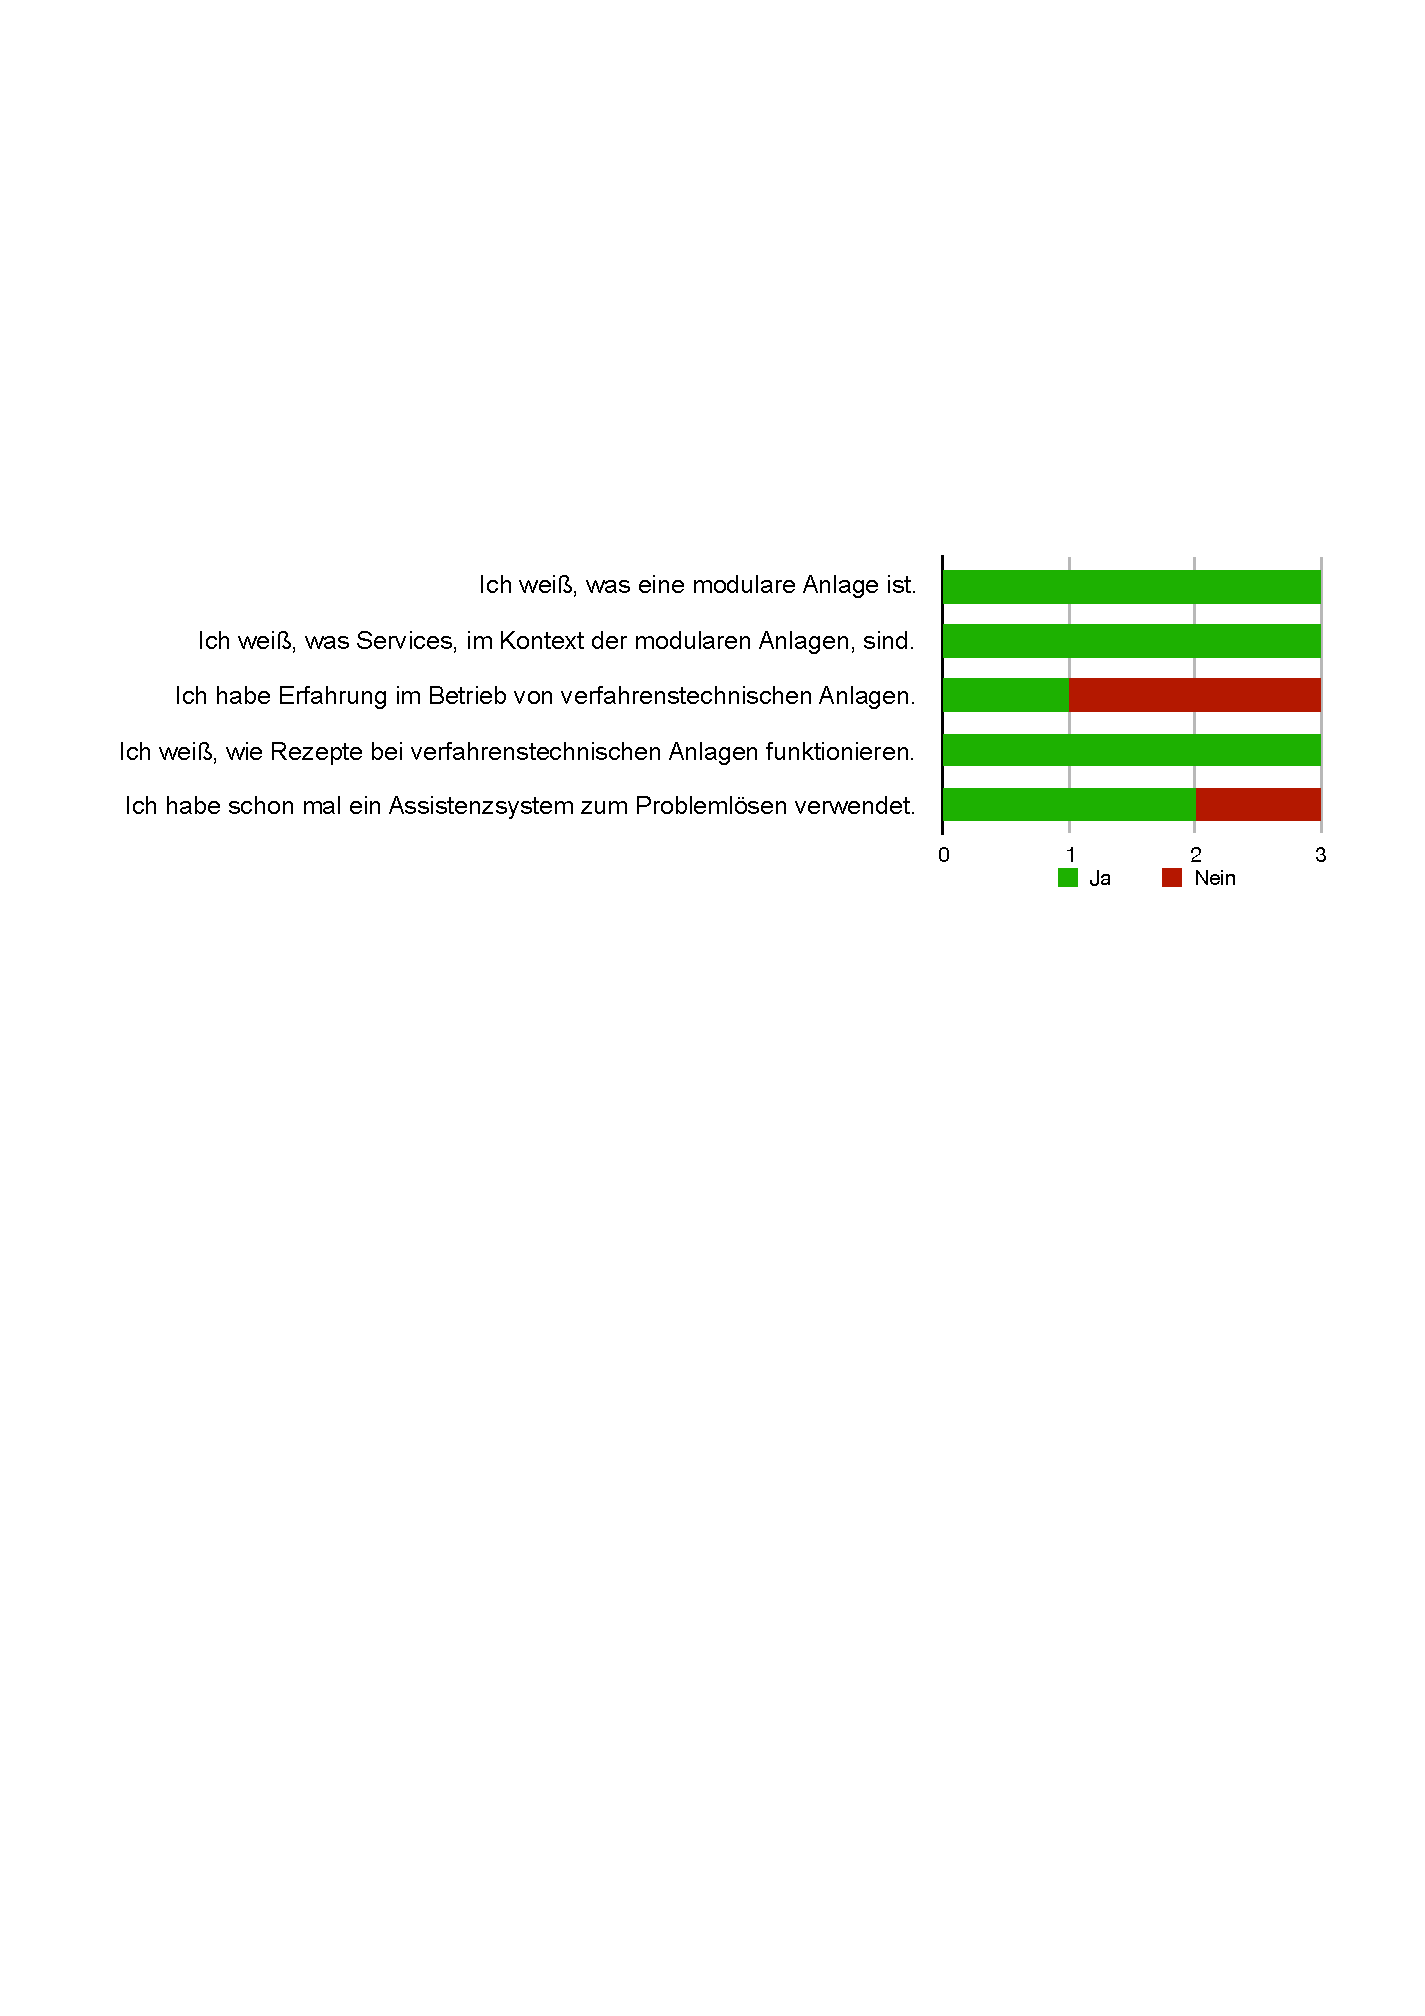
\includegraphics[scale=0.65]{DA_files/Bilder/Validierung/Bild-Vorwissen.pdf}
\caption{Vorwissen zu modularen Anlagen und Assistenzsystemen}
\label{pic:Fragebogen-Vorwissen}
\end{figure}

\begin{figure}[htbp]
\centering

\end{figure}

\subsubsection*{Für gut befunden}
Vorschlag von mehreren Lösungen

Sehr übersichtlich

\subsubsection*{Verbesserungsvorschläge}
Gesamtkosten aufführen -> was kostet ein Mitarbeiter (haben sowohl Luise, als auch Valentin gesagt)

Wunsch: Beim Durchführen der Lösungen unterstützen

Kennt das Assistenzsysteme alle möglichen Lösungen 


\section{Zusammenfassung}
Anforderungen:
Problemidentifikation -> gut erfüllt, es fehlt die Möglichkeit, dass der Nutzer Probleme erstellen kann; noch unklar, welche Informationen das Unternehmen über Produktionsprozess wünscht

Problemlösung -> mäßig erfüllt, da Nutzer keine Lösungen vorschlagen kann, die Auswirkungen auf den Produktionsprozess nicht angezeigt werden (digital Twin)

Klustern

----

Nutzerumfrage